% !TeX root = ../main.tex
% Add the above to each chapter to make compiling the PDF easier in some editors.

\chapter{Background}\label{chapter:background} % Anshul 4 sayfa yazmış

\section{Cloud Computing Landscape} % Cloud usage scenarios
\subsection{Usage Scenarios}
Cloud computing is becoming increasingly popular as on-demand provisioning capabilities and support for various use cases are growing \cite{cloud-use-cases}. Some of those use cases include file storage like OneDrive, database as a service systems like Amazon SimpleDB, entertainment services such as Netflix, multiplayer online games like Dota 2. Businesses are also using cloud computing for instant messaging between departments through applications like Slack or storing customer data in customer relationship management services provided by companies such as SAP or Salesforce. Many businesses also offload their computing requirements to cloud for data mining or for project management as the Pay-per-use model of cloud is very beneficial for companies because they don't need to maintain a cluster of computers on premise. Cloud computing is also being used to host social networks such as Facebook.com or Twitter.com with their massive monthly user counts, 2.45 billion and 330 million, respectively.

\subsection{Virtualization}
The different use cases explained above are only possible because cloud computing provides abstraction by virtualisation. Physical hardware in data centers can be abstracted and be broken to smaller units and can be distributed among customers as virtual machines. This way every customer can have their own personal computer running on the cloud and their system is fully isolated from other customers. While virtual machines were the de facto unit in cloud computing for many years, now there is a new technology called \textit{containerization}. Contaniers allow applications to be packed alongside with their dependencies, and those application can run on the same host OS on top of a container engine. That leads to better utilized servers and less dependency from the underlying hardware. The trade-off is increased delay, because containers add another layer of abstraction on to the stack.

The abstraction in cloud is possible with hypervisor technologies such as Xen. Controlled by software APIs, hypervisors boot self-contained virtual machines on demand, and can run applications as if they were running on physical hosts. This is called \textit{server consolidation} and it has been a great way to reduce under-utilized hardware.

\section{Unikernels}
Unikernels \cite{library-operating-system} \cite{madhavapeddy2014unikernels} are specialised machine images compiled from high-level languages. Those machine images can run directly on the hypervisor or on bare metal. First examples of unikernels can be seen since the late 1990's with the projects like Exodus \cite{exokernel} and Nemesis \cite{nemesis}. In a unikernel project, the developer selects libraries from a repository where the OS functionalities are implemented in. In most cases, these libraries are also implemented in the high-level language that the project is implemented. Once the required libraries for the project are selected, whole codebase is compiled with configuration code for the target runtime. The resulting artifact has the modular stack architecture similar to figure \ref{fig:unikernel-arch} and is a single OS image. This OS image can then be distributed analogous to conventional OS images and be booted directly by a hypervisor or installed to hardware through BIOS. They can be uploaded to cloud systems like OpenStack \cite{openstack} to be booted at will or can be distributed to smaller devices, which is the purpose of this project.

\begin{figure}[htpb]
  \centering
  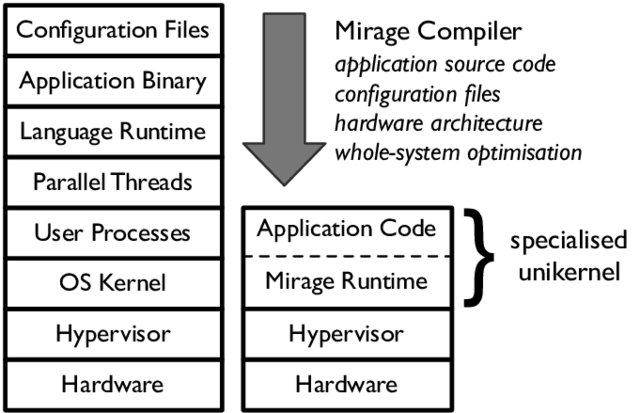
\includegraphics[height=0.3\textwidth]{figures/Contrasting-software-layers-in-existing-VM-appliances-vs-unikernels-standalone-kernel_W640.jpg}
  \caption{ Contrasting software layers in existing VM appliances vs. unikernel’s standalone kernel compilation approach. \cite{library-operating-system}} \label{fig:unikernel-arch}
\end{figure}

Unikernels are currently not production ready \cite{unfit-for-production}. They lack the proper tooling around them and they don't have a "killer-app" for now. However, there is a growing interest around them with startups trying to bring the technology to general usage. One of those startups is Unikernel Systems, based in Cambridge, UK. Unikernel Systems was acquired by Docker in 2016 \cite{docker-acquisiton}. The company consists mostly of developers from the Xen Project. Unikernel technology is more low-level than what Docker provides with its containers and the stated goal of the acquisition is that they want to use the low-level programming expertise of the unikernel team to enhance the power of Docker. All these connections between those three components, namely Docker, Unikernel System and ex-Xen developers show us the big picture of the future cloud technology.

The advantages and drawbacks of using unikernels are explained in the \hyperref[chapter:implementation]{implementation} and \hyperref[chapter:evaluation]{evaluation} part of this thesis with encountered problems and their possible solutions.

The unikernel ecosystem thrives through open source projects. There is currently no production ready unikernel project that can be used for any arbitrary need. There are multiple groups developing unikernel solutions. A small group of these solutions include:
\subsection*{MirageOS}

\url{https://github.com/mirage/mirage} \cite{madhavapeddy2014unikernels}
  MirageOS is a unikernel solution for the OCaml language. It provides libraries for e.g. networking, storage that become operating system drivers when the application is compiled. It produces artifacts that run either on the XEN or KVM hypervisors. It also runs on the ARM64 CPUs, which makes it possible to deploy MirageOS unikernels to Raspberry Pi as IoT targets.
\subsection*{Unik}
\url{https://github.com/solo-io/unik} \cite{levine2016unik} This project brands itself as "Compilation and Deployment Platform" and has support for many providers. It has an API similar to Docker for building unikernels and for managing them. They require a Docker program to be running in the background to manage Unik unikernels properly. They have a wide-range support for different unikernel runtimes such as Osv, MirageOS or Virtualbox. They have a demo of running unikernels on a Kubernetes cluster \cite{unik-youtube}, but there are not instructions to replicate that.
\subsection*{IncludeOS}
\url{https://github.com/includeos/IncludeOS} \cite{7396164}
IncludeOS includes the operating system code to the application as a library when compiled. It can be used to develop C and C++ applications. They target IoT devices as well for improved security. One of their goals is to make IncludeOS bootable on Raspberry Pi M3 B+ models. It supports KVM and some cloud providers such as Google Compute Engine. An IncludeOS image can be booted in tens of milliseconds and only takes 3-4 megabytes in size.

\subsection*{Ops}
\url{https://github.com/nanovms/ops}
  Ops is an interface for creating and managing unikernels in the nanovms infrastructure \cite{nanovms}. It has a wrapper around QEMU \cite{qemu} to run unikernels within the Ops-cli. Ops uses configuration files to embed static content and to configure runtime arguments of images at compile time. It supports multiple languages.
\newline


There is also a new trend in developing unikernels with the Rust programming language. Rust uses modern paradigms for system level programming and that allows young developers to develop unikernel applications without any knowledge of C or OCaml. Lankes et al. are "exploring Rust for Unikernel Development" with detail in \cite{Lankes2019}.

While some of those projects include Kubernetes as their deployment target; they do it by including a host OS, thus does not use the full potential of unikernels.

There are companies working on development of unikernels. The most prominent one is Docker, which is the de facto standard for containerized applications \cite{francia_2016}. Unikernels were also subject to CNCF conferences in the past.

\section{Orchestration}
The adoption of containers in the IT world is still low but it's growing every year. A survey made by Diamante states that \textit{"in 2018 just 17 percent said that IT operations teams were driving container adoption; a year later that number has jumped to more than 35 percent"} \cite{diamante}. They also state that the reason for this big shift is the improvements in orchestration technology. Currently the most popular orchestration technology is Kubernetes, an open source project, initiated by Google. Kubernetes connects multiple machines together and serves their compute resources through a single interface for container deployment. It takes the responsibility of running containers from developers and gives it to automation algorithms. It's treating containers as short-lived entities and deploys them again if a container fails or if a better resource utilization oppurtunity is available.

Kubernetes' popularity comes from the experience of the developers who built it. It's the third generation container-management system\footnotemark developed at Google, a company that has been managing Linux containers for more than ten years \cite{acm-borg}. It grows together with the current trend of microservice architecture, a paradigm that divides bigger applications into smaller units. A Kubernetes cluster can support up to 150,000 pods \cite{kubernetes-load}, Kubernetes' smallest unit. It is very customizable and there are many products on top of it in the Cloud Native Computing Foundation to enhance more of its capabilities. Some of those projects in the ecosystem include, e.g. Istio for service meshing, which allows better customisation of inter-cluster communication, Helm as a package manager for Kubernetes applications or Envoy as a service proxy.
\footnotetext{The main difference between those systems is their API structure. Borg grew organically from the needs of internal teams at Google, thus has an inconsistent API. Omega took successful parts of Borg while providing a centralized access to a consistent API structure. Kubernetes has a more diverse API to help external developers with different needs manage distributed systems.}
Next section explains how Kubernetes works internally and which parts of it are replaced for this thesis.

\subsection*{Kubernetes Architecture}
\begin{figure}[htpb]
  \centering
  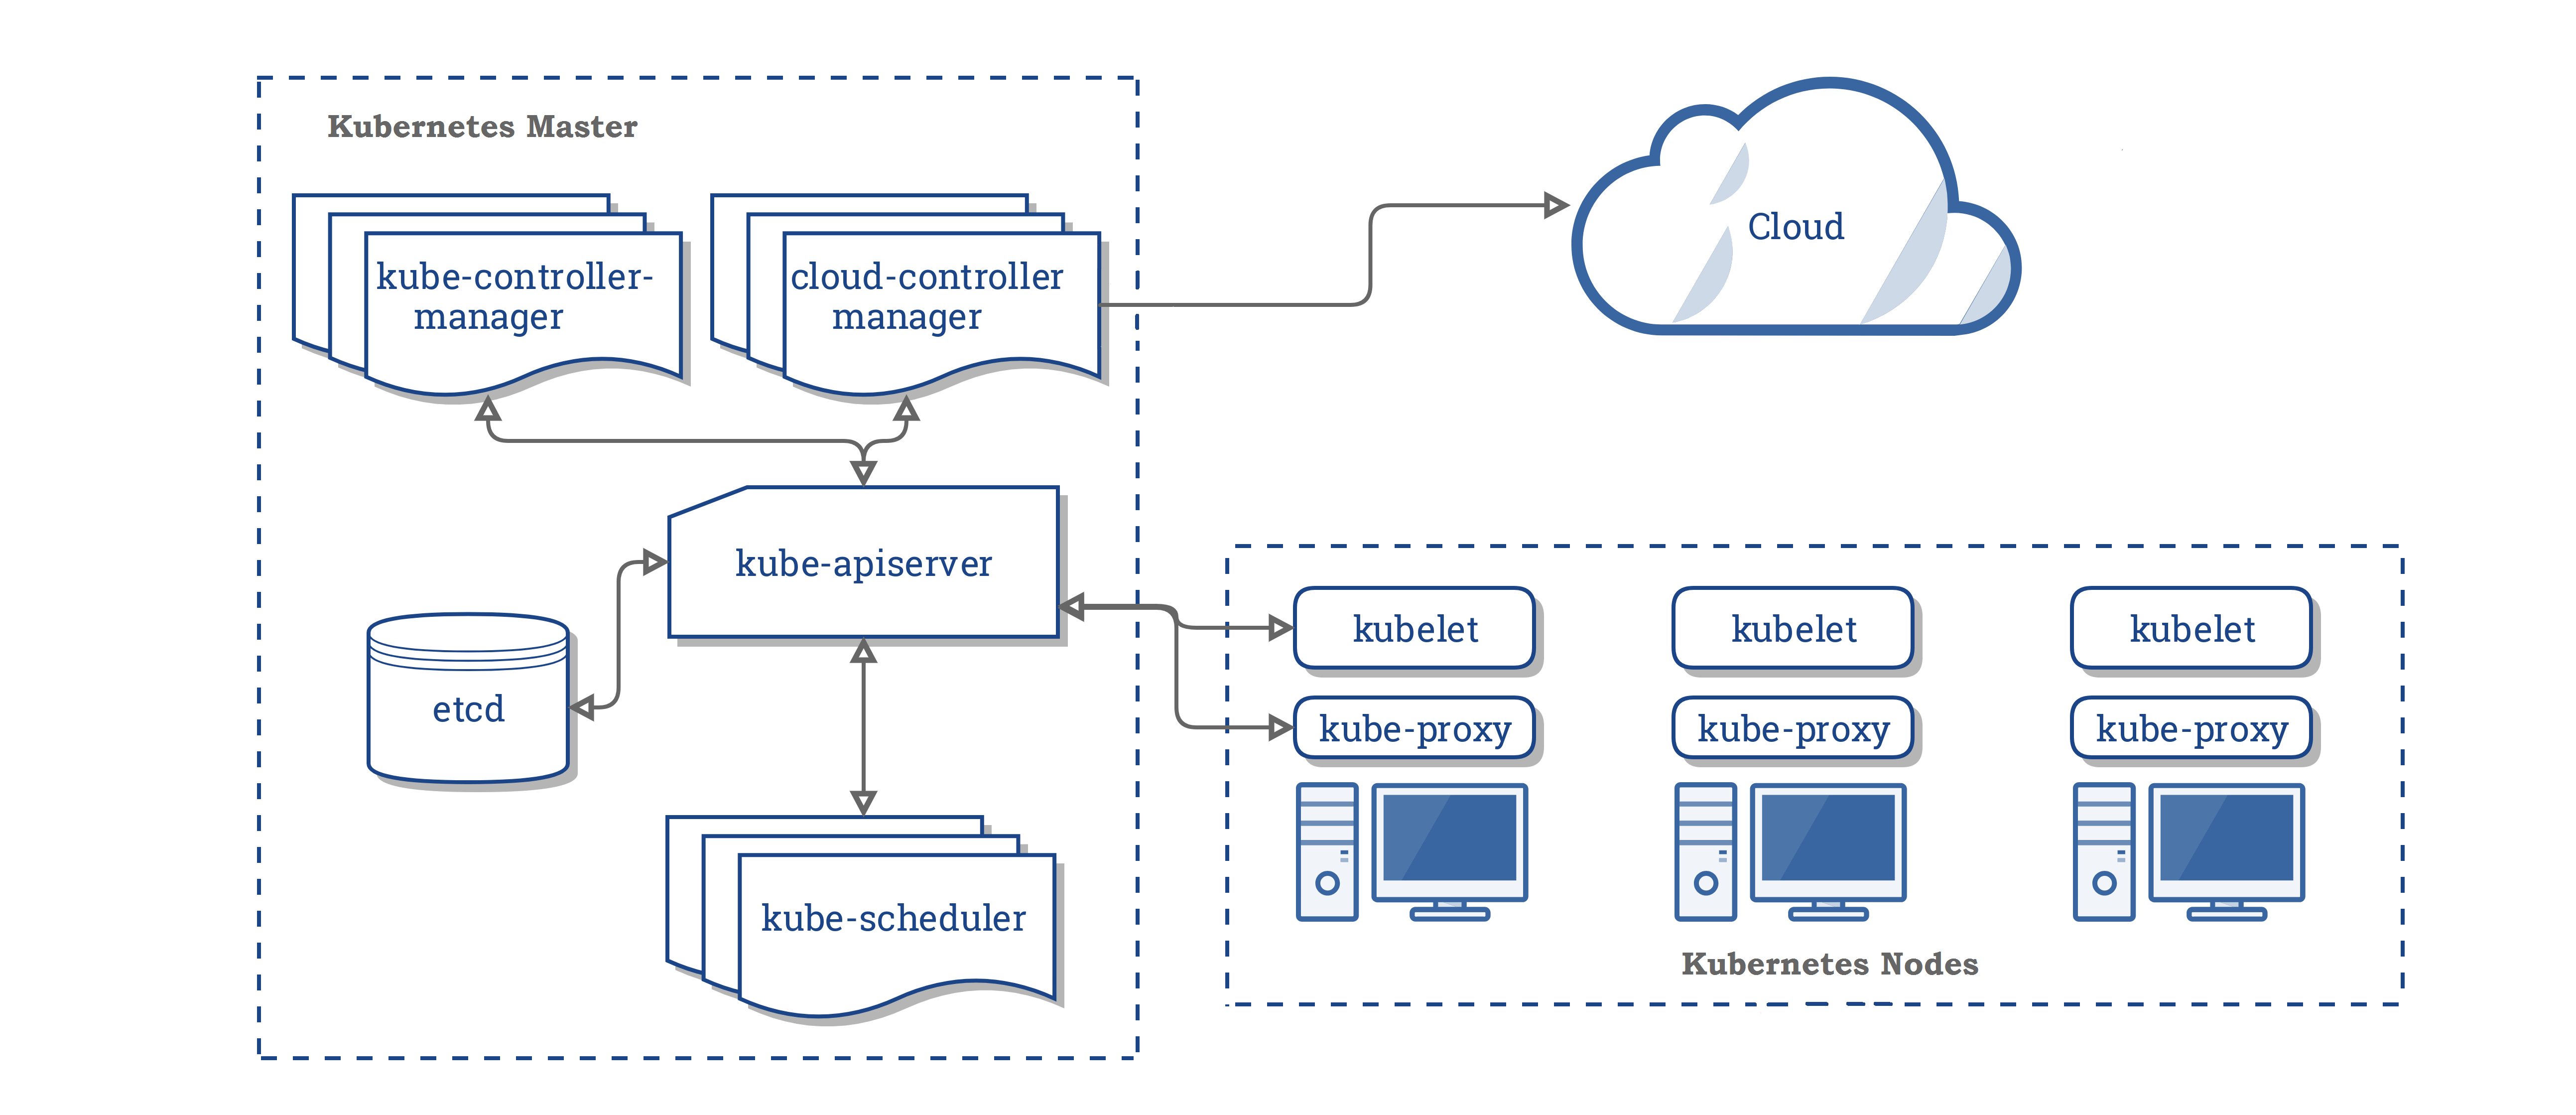
\includegraphics[width=1\textwidth]{karch.png}
  \caption{Kubernetes Architecture \cite{kubewebsite}} \label{fig:kubearch}
  \end{figure}

  A Kubernetes cluster consists of at least one master node and at least one worker node. Figure \ref{fig:kubearch} shows the high level architecture and core components of a Kubernetes cluster with 1 master node and 3 worker nodes. Those core components are explained below. The parentheses near the component's name state on which node they run.

  \subsubsection*{etcd-cluster (master node)}
  Etcd \cite{etcd} is a distributed key-value store developed by CoreOS. It was contributed to Cloud Native Computing Foundation in 2018. Kubernetes uses it to store all its internal state. Etcd notifies other components when cluster's state gets updated. It uses the Raft algorithm \cite{raft} for consensus.

  \subsubsection*{kube-scheduler (master node)}
  Kube-scheduler reacts to new deployments and finds nodes to run those pods. It runs number of algorithms with the data it has. That data includes constraints from the deployment specification such as CPU \& Memory requests, data locality, affinity and the capacity of the nodes. Once a suitable node is found, instead of deploying the pods by itself, scheduler updates the deployment specification and sends it back to the API server.

  It's possible to extend the kube-scheduler either by providing it a config file with custom metrics or by deploying a custom kube-scheduler to the cluster.

  \subsubsection*{kube-controller-manager (master node)}
  Kube-controller-manager runs controllers that work on bringing current state of the cluster to its desired state. Those controllers include Node Controller, Replication Controller, Endpoints Controller, Service Account \& Token Controllers. It watches the API server for changes and reacts to them.


  It's possible to extend Kubernetes by developing new controllers using the operator pattern \cite{operatorpattern}. Operator pattern allows developers to write their own controllers to manage their custom resources. Adding custom resources to Kubernetes is explained in the next chapter. The possibility of deploying a controller for unikernel deployment is investigated in the \hyperref[chapter:implementation]{implementation} chapter.

  \subsubsection*{cloud-controller-manager (master node)}
  Cloud-controller-manager is a new component that is in beta stage for version 1.17 of Kubernetes. It abstracts cloud provider logic from internal Kubernetes logic and allows companies to integrate their infrastructure-related code to Kubernetes through an interface. It allows functions such as checking disconnected nodes, managing cloud provider load balancer for Ingress, managing volumes, etc. Cloud providers such as Digital Ocean, keepalived, Oracle Cloud Infrastructure and Rancher use this approach to manage Kubernetes instances on their cloud. Other providers such as Google or AWS use official cloud provider projects inside the Kubernetes organization for their infrastructure.
  \subsubsection*{kube-apiserver (master node)}

  Kube-apiserver is the frontend component of the control plane that exposes the API. It's the only component that receives updates on internal resources and communicates with the etcd store. It can scale horizontally if there are many requests coming to it; It's also the component that does authentication on these requests.
  \begin{figure}[htpb]
    \centering
    \fbox{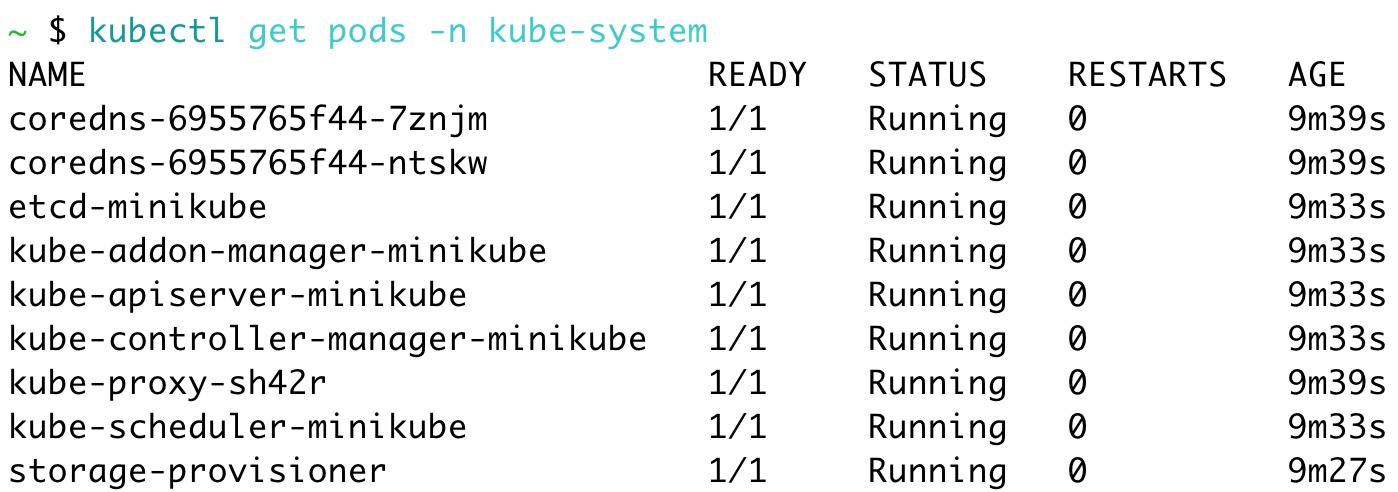
\includegraphics[width=0.9\textwidth]{minikubepods.png}}
    \caption{Management pods runing on a Minikube cluster}\label{fig:minikupods}
  \end{figure}
  
  \subsubsection*{kubelet (every node)}
  Kubelet is a daemon running on every Kubernetes node, including the master node. It manages pod lifecycle on the node. It also provides health check for the node to Kubernetes API and monitors pods for resource consumption. It's responsible for restarting containers if they fail.

  Kubelet is the first component to be replaced in this thesis. By default, it runs Docker containers and this thesis aims to run unikernels without depending on Docker. Because of that Kubelet was replaced with an application called virtual-kubelet. Virtual-kubelet is explained in the next section.
  \subsubsection*{kube-proxy (every node)}
  Kube-proxy runs on every node and maintains networking. It has capabilities to forward network packages for TCP, UDP, SCTP protocols. If the host node has a package filtering layer, kube-proxy uses it for forwarding.

  Kube-proxy is a Docker process, thus can be seen in figure \ref{fig:minikupods} as running. Because this thesis uses a different runtime, it can't be deployed to nodes running the virtual-kubelet instances. While Kubernetes API sends the pod specification to all nodes because of its DaemonSet resource, the deployment is simply ignored by virtual-kubelet. This prevents unikernel deployments from communicating with other resources in the cluster. A solution to th,s problem is to give IPv6 IPs to unikernel instances. This will remove the need for inter-cluster networking and every unikernel will be reachable.

\subsection*{Kubernetes Concepts}
Kubernetes has number of definitions for representing state. Those object definitions help Kubernetes to be portable because in most cases those definitions are stored with the application code together and when migrating to a new cluster, sending them to the new Kubernetes API is enough to achieve the desired state. 

There are more defitions on Kubernetes API but the ones listed here are the most important ones for this thesis.

\begin{description}
  \item [Pod] is the smallest unit in Kubernetes that stores information of how its containers should run in the cluster.
  \item [Service] creates an entry in the internal DNS system and acts as a gateway for a group of pods. Services make pods reachable to other pods without needing their IP addresses. There are 3 different service types. ClusterIP exposes pods only internally. NodePort exposes pods on each node's IP at the given port, makes them reachable with \textit{<NodeIP>:<NodePort>}. LoadBalancerIP exposes pods through cloud provider's load balancer.
  \item [Persistent Volume] is a piece of storage that can be used by other resources. To assign a volume to a pod, Persistent Volume Claim has to be used.
  \item [Labels] are key-value pairs attached to resources for identifying them. In this thesis they are attached to deployments, nodes and DaemonSets to identify unikernel-enabled parts of the cluster.
  \item [Deployment] defines the desired state for a pod. Deployment controller works with the API server to create/destroy containers to achieve that state.
  \item [DaemonSet] is a special kind of deployment that is being deployed to every node on the cluster that fits the requirements. A fresh Kubernetes cluster only has one DaemonSet, kube-proxy.
  \item [Custom Resource Definition (CRD)] is used to extend the Kubernetes API. Users can define their own resources and Kubernetes API serves them through its own REST API.
\end{description}

\subsection*{Kubernetes Alternatives}
Kubernetes is the most dominant product on the market right now as can be seen from figure \ref{fig:kusage} but alternatives exist. Some of those alternatives have a more narrowed focus than Kubernetes, providing less capabilities while being easier to operate. 

\begin{figure}[htpb]
  \centering
  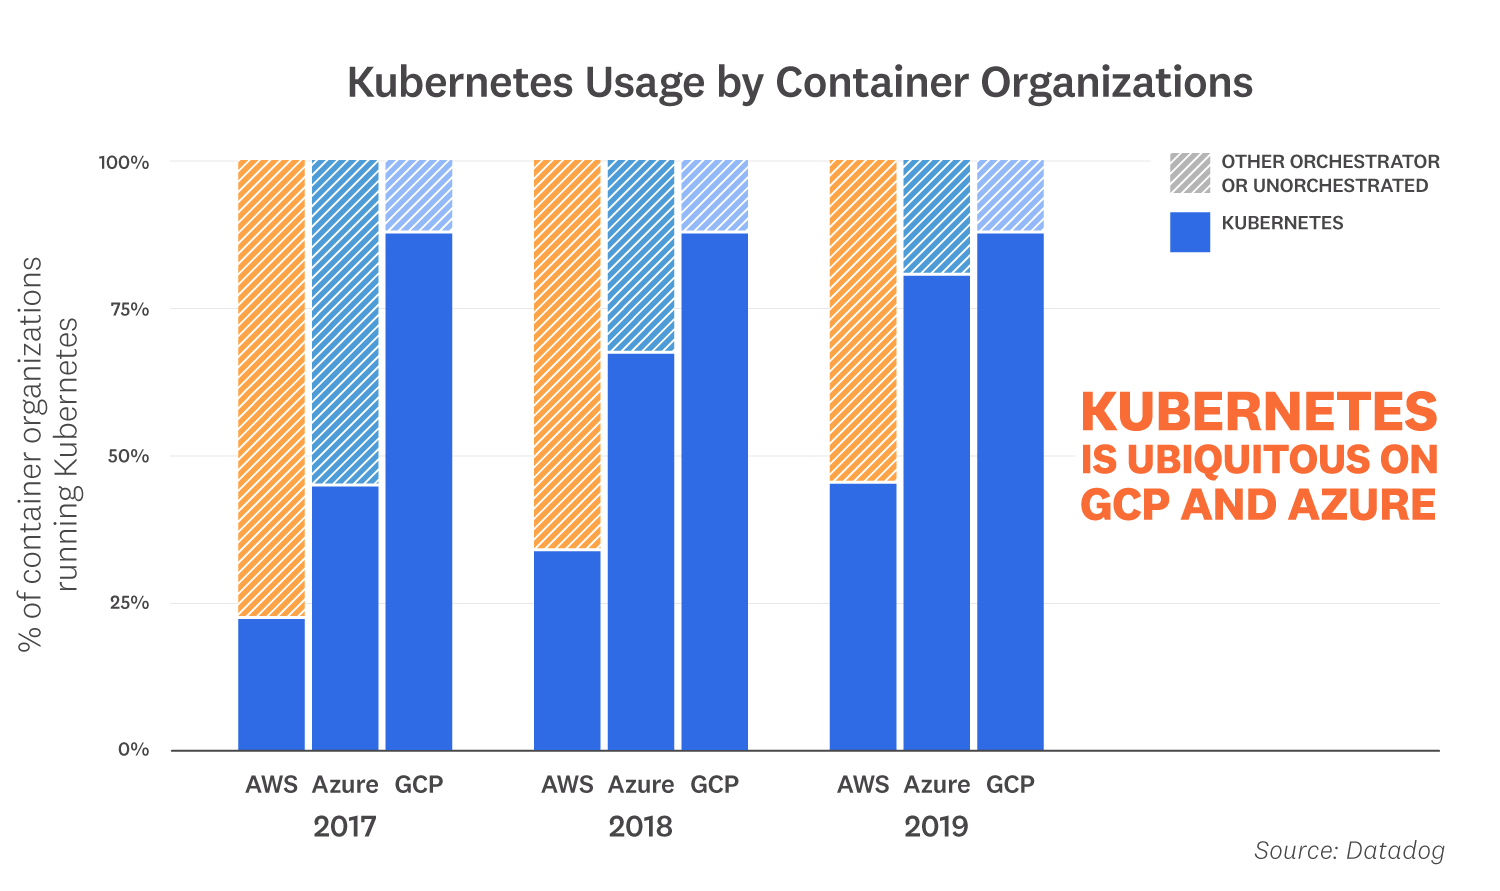
\includegraphics[width=1\textwidth]{kusage.png}\caption{Kubernetes usage by container organizations \cite{datadog}}\label{fig:kusage}
\end{figure}

A small group of these alternatives are as follows:

\subsubsection*{Docker Swarm}
Docker Swarm is the orchestration solution from the Docker company. It uses the same API as the Docker-cli, so users don't need to learn another set of commands. However, it has more limited functionality than Kubernetes. While Kubernetes has APIs to handle different use cases it encountered through the years, Docker Swarm is limited to what Docker can do. If Docker does not support an operation, it's very hard to implement it in Docker Swarm.

\subsubsection*{Apache Marathon}
Apache Marathon is an orchestrator built on top of Mesos. Mesos is a highly scalable resource manager, also from Apache. Marathon provides scaling, self-healing and service discovery for containerized applications on top of Mesos. It can run both Docker containers and Mesos specific containers.

\subsubsection*{HashiCorp Nomad}
Nomad follows the *nix philosophy of \textit{"Do One Thing And Do It Well"}. It provides a single binary both for the server and client, which has a resource manager and a scheduler, while Kubernetes has half a dozen components to operate a fully functioning cluster. Nomad also has support for other runtimes such as standalone applications. It can not provide as good customisation as Kubernetes though.

\section*{Virtual Kubelet}
Virtual-kubelet \cite{virtual} is a project to \textit{masquearade} kubelet component of Kubernetes. It uses the same interface with the upstream kubelet component and can be initialized with the same flags as the normal kubelet instance. When initialized with a valid kubeconfig file, virtual-kubelet introduces itself as a valid node to the Kubernetes API and awaits commands from it. The project is initiated by Microsoft to offload their Kubernetes workload to their Azure Container Instances. It's now an official Cloud Native Computing Foundation (CNCF) project.

Virtual-kubelet implements core parts of kubelet and achieves custom business logic through providers. The provider interface allows developers to implement their own logic for creating workloads with the data provided by Kubernetes Pod specification. In Azure's case, they have a provider that users configure with their Azure credentials and when a new pod specification comes, virtual-kubelet deploys the Docker containers to Azure Container Instances through the official Microsoft Azure API. Users never have to interact with the Container Instances service outside the Kubernetes API and if they want to scale their deployment, they do it through the Kubernetes API. Virtual-kubelet runs the respective functions to correct the number of instances running on Container Instances. Those functions are explained more in \hyperref[chapter:implementation]{implementation}.

Virtual-kubelet does not support some of the kubelet functions such as volume mounting or networking. Those functions have to be integrated by the provider developer. In Azure's case only stateless applications can be deployed to Container Instances and they have to communicate through a public endpoint if they want to communicate with other services in the cluster. Microsoft demonstrates their usage of virtual-kubelet by deploying a job that pulls images from its Azure Storage service that lives outside the Kubernetes cluster; labels the images; uploads them back to Azure Storage Service. The job is stateless and only communicates with the public Azure Storage endpoint through valid credentials. To label more images in parallel, the job is scaled through the Kubernetes API.

There are other officially supported providers as well. Alibabacloud Elastic Container Instance, AWS Fargate, OpenStack Zun Container service, HashiCorp Nomad \& Huawei Cloud container Instance have providers for virtual-kubelet. A pattern that can be seen here is that other than Nomad, all those providers are Container Instances provided by different cloud companies. Their use-cases are similar to Azure's. Their examples only deploy one virtual-kubelet instance to the cluster and they provide their serverless container services through it. This whole workflow can be summarised by saying that virtual-kubelet allows seamless integration with other orchestrators that support similar functions to Kubernetes.

The virtual-kubelet repository also contains a provider for running containers in \textit{containerd} runtime. That provider differs itself from other examples by being deployed to a server other than the cluster. It still uses the CRI API provided by Kubernetes for managing containers. That allows it to run the same Docker container given to it from the Pod specification because Docker also uses \textit{containerd} underneath. The similarity between that provider and the provider presented in this thesis is that they are both being deployed not to the cluster but to the servers. The difference between them is this thesis manages unikernels and does not require any container runtime to operate.

The virtual-kubelet version used for this thesis is 1.0.0. At the time of writing, the latest version was 1.2.1.
\section{Managing IoT}
It's expected that there will be "20 billion to 35 billion" \cite{unikernels-improve} connected devices in 2020. There are different initiatives to manage this complexity caused by the number of devices out there. Amazon provides device software, connectivity tools and analytics services to their customer to use on their IoT scenarios. Google, like Amazon, provides an IoT Core, a complete pipeline for managing devices and collecting data. While those solutions work, they have a vendor lock-in problem. IoT software is mostly embedded and it's a cumbersome job to move from one software to another one when changing providers. The IoT industry is still a young industry and it lacks unified protocols that are shared by companies providing those services.

A project called K3S \cite{k3s} is a step towards the direction to unify IoT communication. K3S is a Kubernetes distribution aimed for IoT \& edge computing. It supports ARM architecture and can be deployed to a Raspberry Pi device. It can be used to create a connected cluster between a K3S master running in the cloud and IoT devices acting as secondary nodes. K3S uses a modified version of the Kubernetes' codebase. The modifications include using \textit{sqlite} as the default storage mechanism instead of \textit{etcd}; packaging required external dependencies with the application; removing cloud provider specific storage plugins. All those modifications aim to provide a single binary for the cluster. Despite using the same codebase, it can't be used together with a normal Kubernetes cluster. That restricts its wide adaption. A company aiming to connect IoT devices through K3S, has to have a K3S deployment on their infrastructure. If they have a Kubernetes cluster for their infrastructure, those clusters can only communicate externally.

Microsoft Azure allows virtual-kubelet to be used with their IoT solutions and with their Kubernetes services \cite{Chandra2019}. A virtual-kubelet instance translates Kubernetes deployment specification to IoT Edge specification, then submits it to the Azure IoT hub. This project "does not provide Kubernetes-backed high availability or disaster recovery to IoT Edge deployments" \cite{azure-vk-github}. Both in Azure's case and in the research proposed by FLEDGE \cite{fledge}, virtual-kubelet was deployed on the cloud and acted as a middle-man between Kubernetes and IoT based communication.